\documentclass[a4paper,12pt]{report}
\usepackage{graphicx}
\usepackage{hyperref}
\usepackage[T1]{fontenc}
\usepackage[utf8]{inputenc}
\usepackage[english,italian]{babel}
\usepackage{setspace}
\usepackage[paper=a4paper,margin=1in]{geometry}
\usepackage{lipsum}
\usepackage{microtype}
\usepackage{times}
\usepackage{xcolor}
\usepackage{hyperref}
\usepackage{float}
\graphicspath{ {images/} }

\title{Test Document}
\author{Simone Renzo}
\date{Febbraio 2021}

%%%%********************************************************************
% fancy quotes
\definecolor{quotemark}{gray}{0.7}
\makeatletter
\def\fquote{%
	\@ifnextchar[{\fquote@i}{\fquote@i[]}%]
}%
\def\fquote@i[#1]{%
	\def\tempa{#1}%
	\@ifnextchar[{\fquote@ii}{\fquote@ii[]}%]
}%
\def\fquote@ii[#1]{%
	\def\tempb{#1}%
	\@ifnextchar[{\fquote@iii}{\fquote@iii[]}%]
}%
\def\fquote@iii[#1]{%
	\def\tempc{#1}%
	\vspace{1em}%
	\noindent%
	\begin{list}{}{%
			\setlength{\leftmargin}{0.1\textwidth}%
			\setlength{\rightmargin}{0.1\textwidth}%
		}%
		\item[]%
		\begin{picture}(0,0)%
			\put(-15,-5){\makebox(0,0){\scalebox{3}{\textcolor{quotemark}{``}}}}%
		\end{picture}%
		\begingroup\itshape}%
	%%%%********************************************************************
	\def\endfquote{%
		\endgroup\par%
		\makebox[0pt][l]{%
			\hspace{0.8\textwidth}%
			\begin{picture}(0,0)(0,0)%
				\put(15,15){\makebox(0,0){%
						\scalebox{3}{\color{quotemark}''}}}%
		\end{picture}}%
		\ifx\tempa\empty%
		\else%
		\ifx\tempc\empty%
		\hfill\rule{100pt}{0.5pt}\\\mbox{}\hfill\tempa,\ \emph{\tempb}%
		\else%
		\hfill\rule{100pt}{0.5pt}\\\mbox{}\hfill\tempa,\ \emph{\tempb},\ \tempc%
		\fi\fi\par%
		\vspace{0.5em}%
	\end{list}%
}%
\makeatother
%%%%********************************************************************

\begin{document}
	
	\begin{titlepage}
		\noindent
		\begin{minipage}[t]{0.19\textwidth}
			\vspace{-4mm}{
\includegraphics[scale=1.15]{logo_unimib.pdf}}
		\end{minipage}
		\begin{minipage}[t]{0.81\textwidth}
			{
				\setstretch{1.42}
				{\textsc{Università degli Studi di Milano - Bicocca}} \\
				\textbf{Scuola di Scienze} \\
				\textbf{Dipartimento di Informatica, Sistemistica e Comunicazione} \\
				\textbf{Corso di laurea in Informatica} \\
				\par
			}
		\end{minipage}
		
		\vspace{40mm}
		
		\begin{center}
			{\LARGE{
					\setstretch{1.2}
					\textbf{DevOps: studio e implementazione \\ di una pipeline di CI e CD \\ nel progetto Sphere}
					\par
			}}
		\end{center}
		
		\vspace{40mm}
		
		\noindent
		{\large \textbf{Relatore:} Prof. Mariani Leonardo} \\
		
		\noindent
		{\large \textbf{Tutor Aziendale:} Dott. Mesiano Cristian}
		
		\vspace{15mm}
		
		\begin{flushright}
			{\large \textbf{Relazione della prova finale di:}} \\
			\large{Renzo Simone} \\
			\large{Matricola 781616} 
		\end{flushright}
		
		\vspace{40mm}
		\begin{center}
			{\large{\bf Anno Accademico 2019-2020}}
		\end{center}
		
		\restoregeometry
		
	\end{titlepage}
	
	\selectlanguage{english}
	\begin{abstract}
		In un mondo in continuo sviluppo, la necessità di adattarsi velocemente al cambiamento è spesso
		ciò che permette di contraddistinguere realtà di successo dalle fallimentari.
		Il software è probabilmente uno dei prodotti che più segue questa filosofia di cambiamento repentino,
		con la continua uscita di nuove tecnologie, nuove metodiche e la conseguente necessità di cambiare spesso
		rotta e requisiti in base alle necessità o al mercato di riferimento.
		
		La nascita di metodi \emph{Agile} e di nuove filosofie improntate all'unire ciò che prima era separato,
		in un unico processo, hanno permesso di adattarsi con successo ai cambiamenti, rendendo l'industria del
		software quella più all'avanguardia e resiliente nel tempo, continuando tutt'oggi a migliorarsi sempre più.
		
 		\begin{fquote}[Charles Darwin]
		 	It is not the strongest of the species that survives, nor the most intelligent that survives.
		 	It is the one that is the most adaptable to change.
	 	\end{fquote}
	\end{abstract}

	\selectlanguage{italian}
	\tableofcontents
	
	\chapter{Introduzione}
	
	\section{Il Contesto Aziendale}
	
		\subsection{Storia}
		
			\lipsum[1]
		
		\subsection{Il progetto Sphere}
		
			In un mondo dove l'informazione risiede principalmente sotto forma di immagini, Sphere si propone come soluzione per trasformare il fisico in digitale, rompendo la barriera che divide una semplice fotografia da un 
			elemento tangibile.
			
			\begin{figure}[h]
				\centering
				
\includegraphics[width=0.4\textwidth]{logo_sphere}
				\caption{Sphere Logo}
				\label{fig:logo_sphere}
			\end{figure}
			
			Grazie a Sphere l'utente è in grado di creare un \emph{Digital Inventory} di casa propria, partendo da delle semplici fotografie panoramiche acquisite da lui stesso analizzate e convertite poi in oggetti reali grazie ai modelli di AI che permettono di riconoscere oggetti, materiali e ambienti in modo dinamico. Questi dati possono essere sfruttati specialmente a fini di \emph{risk-management} in ambito assicurativo, velocizzando il processo di \textbf{digital claim management}, quoting e premio assicurativo, attraverso un indice dinamico di "bontà" dell'utenza chiamato \emph{Sphere Index}.\\*
			
			Sphere non è un prodotto unico ma un prodotto \textbf{modulare}, ogni cliente può quindi personalizzare la propria esperienza integrando i moduli necessari al proprio business, senza preoccuparsi di dipendenze esterne o di costi non controllabili.
	
		\subsection{Profilo personale in azienda}
		
			In PerceptoLab Srl, il candidato è stato assunto in Giugno 2020, con ruolo di Infrastructure \& DevOps Engineer, integrato nel team di Backend Development.
	
	\section{Scopo del Project Work}
	
		\subsection{Obiettivi}
	
			Il Project Work ha come scopo il design e l'implementazione di un processo che includa una Pipeline di Continuous
			Integration e di Continuous Delivery, nell'ambito del progetto Sphere.
			
			In particolare si prefigge questi obiettivi:
			\begin{enumerate}
				\item Creazione di un processo di \emph{Continuous Integration} per il repository progettuale, mediante l'uso di tool per il testing automatico e per la gestione delle Pull Request, con integrazione per build in ambiente macOS;
				\item Creazione di un processo di \emph{Continuous Delivery} per la creazione di immagini Docker mediante utilizzo di tag specifici su repository e delivery degli artefatti su registry remoto;
				\item Integrazione nella pipeline DevOps di \emph{analisi statica e dinamica} del codice mediante tools dedicati e definizione di quality gates in base alle necessità progettuali;
				\item Creazione e gestione dell'infrastruttura (basata su \emph{Amazon Web Services}) necessaria al deployment dei servizi sviluppati nel progetto aziendale.
			\end{enumerate}
	
		\subsection{Pianificazione del Lavoro}
	
			Il Project Work si è svolto durante il periodo di 3 mesi tra l'1 Ottobre 2020 ed il 31 Dicembre 2020, in modalità di remote
			working con l'utilizzo di tools di collaboration integrati in Google GSuite (Google Chat, Meets) e nella suite Atlassian
			(Bitbucket, Jira, Confluence).
			
			% TODO: Inserire un GANTT.
	
		\subsection{Prodotti Finali}
		
			I prodotti del project work saranno i seguenti:
			\begin{itemize}
				\item Analisi dei Requisiti per i processi da implementare
				\item Pipeline di Continuous Integration per i servizi di Backend e Mobile
				\item Pipeline di Continuous Delivery per i servizi di Backend (Docker Containers)
				\item Quality Assurance Gates basati sulla analisi dei test e del codice con tools dedicati
				\item Infrastruttura basata su Amazon Web Services (Risorse Cloud, VMs) per gestire i processi descritti.
			\end{itemize}
	
	\chapter{Modelli di Sviluppo del Software}
	
		\section{Il ciclo di vita del software}
	
			\begin{figure}[h]
				\centering
				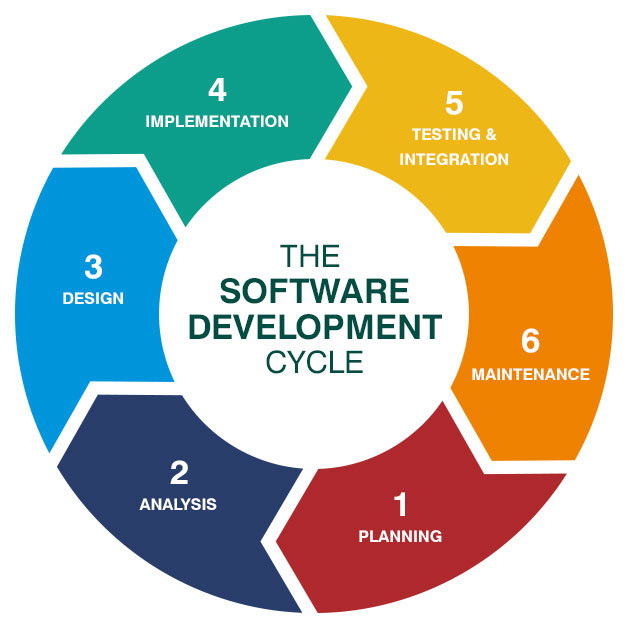
\includegraphics[width=0.4\textwidth]{sdlc}
				\caption{Software Development Lifecycle}
				\label{fig:sdlc}
			\end{figure}
	
			\subsection{Le fasi del ciclo di vita}
	
				Il ciclo di vita del software si riferisce ad una metodologia che permetta di ottenere software di massima qualità
				al minimo costo di produzione e nel minor tempo possibile, dividendo la sua vita in diverse fasi consequenziali:
				\begin{enumerate}
					\item Planning e Analisi
					\item Design
					\item Implementazione
					\item Testing e Integrazione
					\item Manutenzione
				\end{enumerate}
				
				\paragraph{Planning e Analisi}
				Si analizzano i sistemi esistenti per i cambiamenti necessari ed il problema da risolvere in termini di software development.
				Questa fase crea in output una serie di \emph{Requisiti} che possono essere Funzionali, Non Funzionali, o di Dominio, ed un piano
				di lavoro per sviluppare tali requisiti in un tempo definito (ma, come vedremo, variabile in metodi \emph{Agile}).
				Le definizioni di tali requisiti sono dettate dallo standard \href{https://standards.ieee.org/standard/610_12-1990.html}{\emph{IEEE 610.12-1990}}.
				
				\paragraph{Design}
				I requisiti vengono trasformati in una \emph{specifica di Design} (architetturale ed implementativa), che verrà in seguito analizzata dagli \emph{stakeholders}, ottenendo così feedback e suggerimenti in base alle esigenze. In questa fase diventa cruciale implementare un sistema per incorporare i feedback così da migliorare il design finale ed evitare costi aggiuntivi a fine sviluppo.
				
				\paragraph{Implementazione}
				Questa fase inizia lo sviluppo del software in se, seguendo la specifica di design della fase precedente, ed utilizzando convenzioni, code style, pratiche e linee guida comuni per tutti i soggetti coinvolti nello sviluppo. L'utilizzo di linee guida comuni permette di evitare fraintendimenti all'interno del team di sviluppo, e di facilitare le fasi future di manutenzione.
				
				\paragraph{Testing e Integrazione}
				Il software sviluppato viene sottoposto a test per difetti e mancanze, risolvendo i problemi trovati lungo il percorso e migliorando le feature implementate fino ad arrivare ad una qualità in linea con le specifiche originali. In seguito, viene integrato con il resto dell'ambiente mediante deployment, così da poterlo iniziare ad utilizzare in casi reali.
				
				\paragraph{Manutenzione}
				Alla fine del processo, difficilmente si saranno raggiunti tutti i requisiti alla perfezione, motivo per cui la fase di manutenzione gioca un ruolo fondamentale per gestire tutto ciò che segue lo sviluppo principale del software. Questa fase permette quindi di analizzare i comportamenti sul campo del software sviluppato, così da agire di conseguenza nel risolvere problemi in modo più mirato.
	
			\subsection{I modelli classici: Waterfall e Iterativo}
			
				\begin{figure}[h]
					\centering
					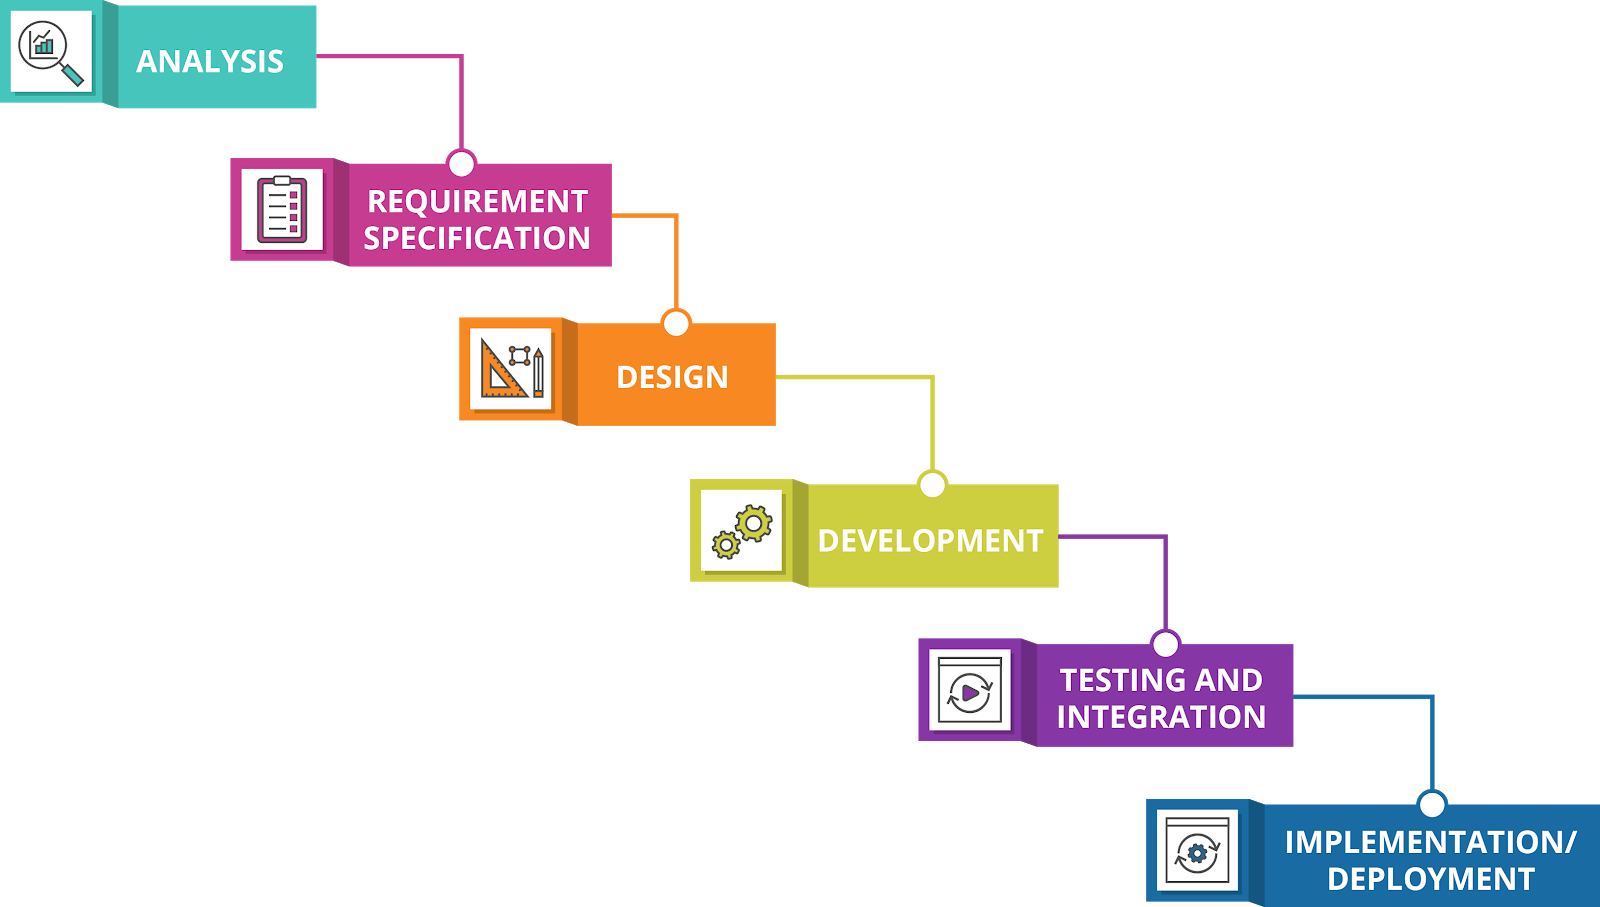
\includegraphics[width=0.8\textwidth]{waterfall}
					\caption{Modello Waterfall}
					\label{fig:waterfall}
				\end{figure}
				
				\paragraph{Waterfall}
				Il processo di sviluppo storicamente più tradizionale e semplice è chiamato \emph{Waterfall}.
				Il nome suggerisce come, rispetto alle fasi del ciclo di vita del software, queste vengano eseguite in "cascata", dove la fine di una fase permette di iniziare quella successiva, seguendo ciò che era stato appreso dalla produzione manufatturiera applicandolo in ambito dello sviluppo software.
				
				\vspace{5mm}
				La creazione di tale processo ha permesso di superare i limiti del processo \emph{code and fix}, permettendo di pianificare in modo più strutturato e dividendo in modo netto le problematiche in base alla fase di appartenenza.
				Altrettante sono però state le problematiche derivanti dalla sua applicazione, tra cui:
				\begin{itemize}
					\item Le fasi di \emph{alpha/beta} testing ripercorrono per natura tutte le fasi del processo, rallentando lo sviluppo;
					\item Ogni fase viene congelata dopo la sua fine, rendendo impossibile la comunicazione tra clienti e sviluppatori dopo la fase iniziale;
					\item La pianificazione viene effettuata solo all'inizio, orientando lo sviluppo ad una data specifica di rilascio; Ogni errore porta a ritardare tale data, che non può però essere stimata di nuovo;
					\item La stima dei costi e delle risorse si rende difficile senza la prima fase di Analisi;
					\item La specifica di requisiti vincola il prodotto da sviluppare, mentre nei casi reali spesso le necessità del cliente cambiano in corso d'opera, specialmente sul lungo termine;
				\end{itemize}
	
				\begin{figure}[h]
					\centering
					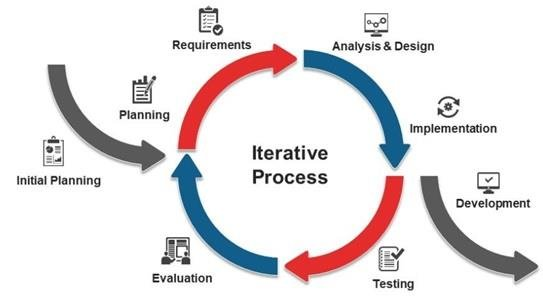
\includegraphics[width=0.6\textwidth]{iterative}
					\caption{Modello Iterativo}
					\label{fig:iterative}
				\end{figure}
	
				\paragraph{Iterativo}
				Una evoluzione del processo \emph{Waterfall} è il modello \emph{Iterativo}, basato sullo stesso ciclo di vita descritto precedentemente, ma con un sostanziale cambiamento che lo rende la base dei modelli odierni, ovvero il riconoscimento che lo sviluppo di un software non è composto di una singola iterazione del flusso ma di diverse iterazioni, sempre incrementali.
				
				\vspace{3mm}
				L'idea alla base del modello \emph{Iterativo} consta nel ripetere il ciclo di sviluppo più volte, in porzioni di tempo più ristrette, permettendo agli sviluppatori di apprendere dai cicli precedenti e di migliorare i successivi, grazie alla continua revisione dei requisiti e del design del software.
				
				\vspace{3mm}
				Il processo parte con una prima iterazione volta a creare un prodotto basilare ma usabile, in modo da raccogliere il feedback dell'utente o cliente da utilizzare come input per il ciclo successivo. Per guidare le varie iterazioni, si sfrutta una lista di tasks necessari per lo sviluppo del software, che include sia nuove feature sia modifiche al design provenienti da iterazioni precedenti, da aggiornare in ogni fase di analisi (per ogni iterazione).
				
				Confrontato con \emph{Waterfall}, il modello \emph{Iterativo} porta diversi vantaggi:
				\begin{itemize}
					\item L'utente viene coinvolto ad ogni iterazione, migliorando il feedback e la qualità del prodotto finale;
					\item Ogni iterazione incrementale produce un \emph{deliverable} che può essere accettato dall'utente, e solo dopo ciò si potrà procedere alla prossima iterazione;
					\item Ogni iterazione permette di rimodulare le risorse necessarie allo sviluppo, così da attuare tecniche di cost-saving;
					\item Il prodotto può essere consegnato fin dalla prima iterazione, seppur in fase embrionale ma funzionante;
					\item Il modello \emph{Iterativo} può essere applicato anche a progetti di piccole dimensioni con successo.
				\end{itemize}
	
		\section{Modelli \emph{Agile}}
	
			\begin{figure}[h]
				\centering
				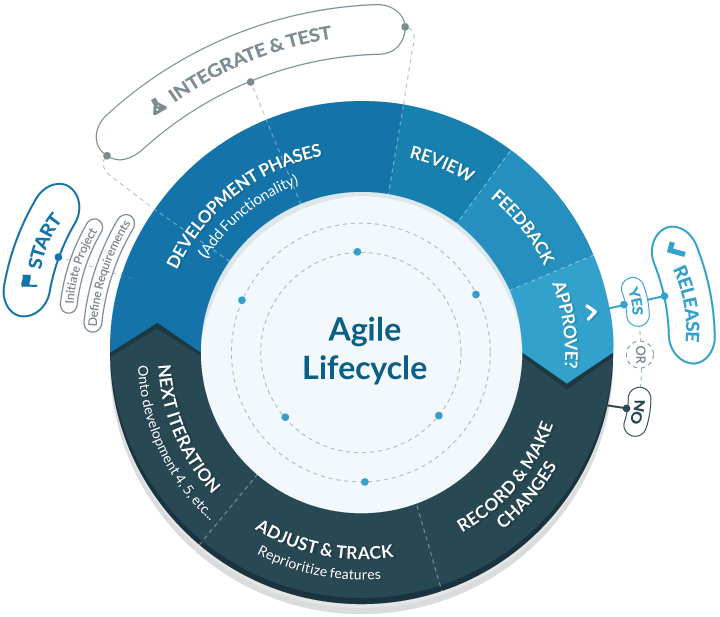
\includegraphics[width=0.8\textwidth]{agile}
				\caption{Modello Agile Generico}
				\label{fig:agile_generic}
			\end{figure}
	
			\subsection{La filosofia \emph{Agile}}
				
				La filosofia \emph{Agile} è emersa a partire dai primi anni 2000, grazie alla pubblicazione del \href{https://agilemanifesto.org/iso/it/principles.html}{\emph{"Manifesto for Agile Software Development"}} nel 2001, nato dall'evoluzione dei metodi classici iterativi ed incrementali.
				
				L'utilizzo di questa filosofia permette di ridurre sensibilmente il rischio di errori dovuti alla male interpretazione dei requisiti o il ritardo nelle tempistiche di consegna del prodotto finale, ponendo il focus sulla \textbf{adattabilità} dei processi al cambiamento e sulla \textbf{soddisfazione} del cliente come metrica di successo di un processo di sviluppo.
				Ciò è permesso grazie alla suddivisione dello sviluppo in \textbf{iterazioni} di piccole dimensioni (generalmente 1-3 settimane), permettendo un rilascio continuo del software in modo incrementale, e dall'attuazione di alcuni principi tra cui:
				
				\begin{itemize}
					\item \textbf{Individui e interazioni}: nello sviluppo \emph{Agile}, auto-organizzazione e motivazione sono importanti tanto quanto le interazioni tra persone e il pair programming;
					\item \textbf{Software Funzionante}: viene consegnato frequentemente software funzionante in tempi preferibilmente brevi, sotto forma di \emph{Demo};
					\item \textbf{Collaborazione col Cliente}: committenti a sviluppatori devono lavorare insieme quotidianamente per tutta la durata del progetto;
					\item \textbf{Risposta al Cambiamento}: lo sviluppo \emph{Agile} si concentra nel fornire una risposta veloce ai cambiamenti nei requisiti, anche in fasi avanzate dello sviluppo;
					\item \textbf{Gestione delle Priorità}: lo sviluppo inizia solo dopo aver messo in priorità gli obiettivi, spesso utilizzando una tecnica chiamata \emph{MoSCoW} (\emph{Must - Should - Could - Won't Have});
					\item \textbf{Timeboxing}: suddividere il progetto di sviluppo in intervalli temporali ben definiti, spesso di pochi giorni o settimane, entro il quale consegnare alcune features, contenuti in intervalli più lunghi di consegna del prodotto finale o di una parte di esso.
				\end{itemize}
			
				I modelli \emph{Agile} presentano diversi vantaggi che han permesso la loro adozione nella maggior parte degli ambienti di sviluppo software, tra cui:
				\begin{itemize}
					\item I processi sono molto \textbf{realistici} e riflettono il mercato;
					\item Promuovono il lavoro in team e il cross-training;
					\item Le funzionalità vengono sviluppate velocemente e dimostrate al cliente;
					\item Utilizzabili sia con requisiti fissati che in continuo cambiamento;
					\item Pianificazione ridotta al minimo;
					\item Facilità di gestione.
				\end{itemize}
			
				Contemporaneamente portano anche alcuni svantaggi, derivanti dalla flessibilità del processo e quindi dalla non applicabilità in tutti i casi esistenti:
				\begin{itemize}
					\item Difficoltà di gestione di dipendenze complesse;
					\item Rischio aumentato sulla sostenibilità e mantenibilità del processo;
					\item Necessità di un piano di lavoro generale, e di \textbf{figure chiave} per far funzionare il processo;
					\item Forte dipendenza dal feedback del cliente, per colpa di cui il team potrebbe essere direzionato in modo errato.
				\end{itemize}
	
			\subsection{Un caso di successo: SCRUM Framework}
			
				\begin{figure}[h]
					\centering
					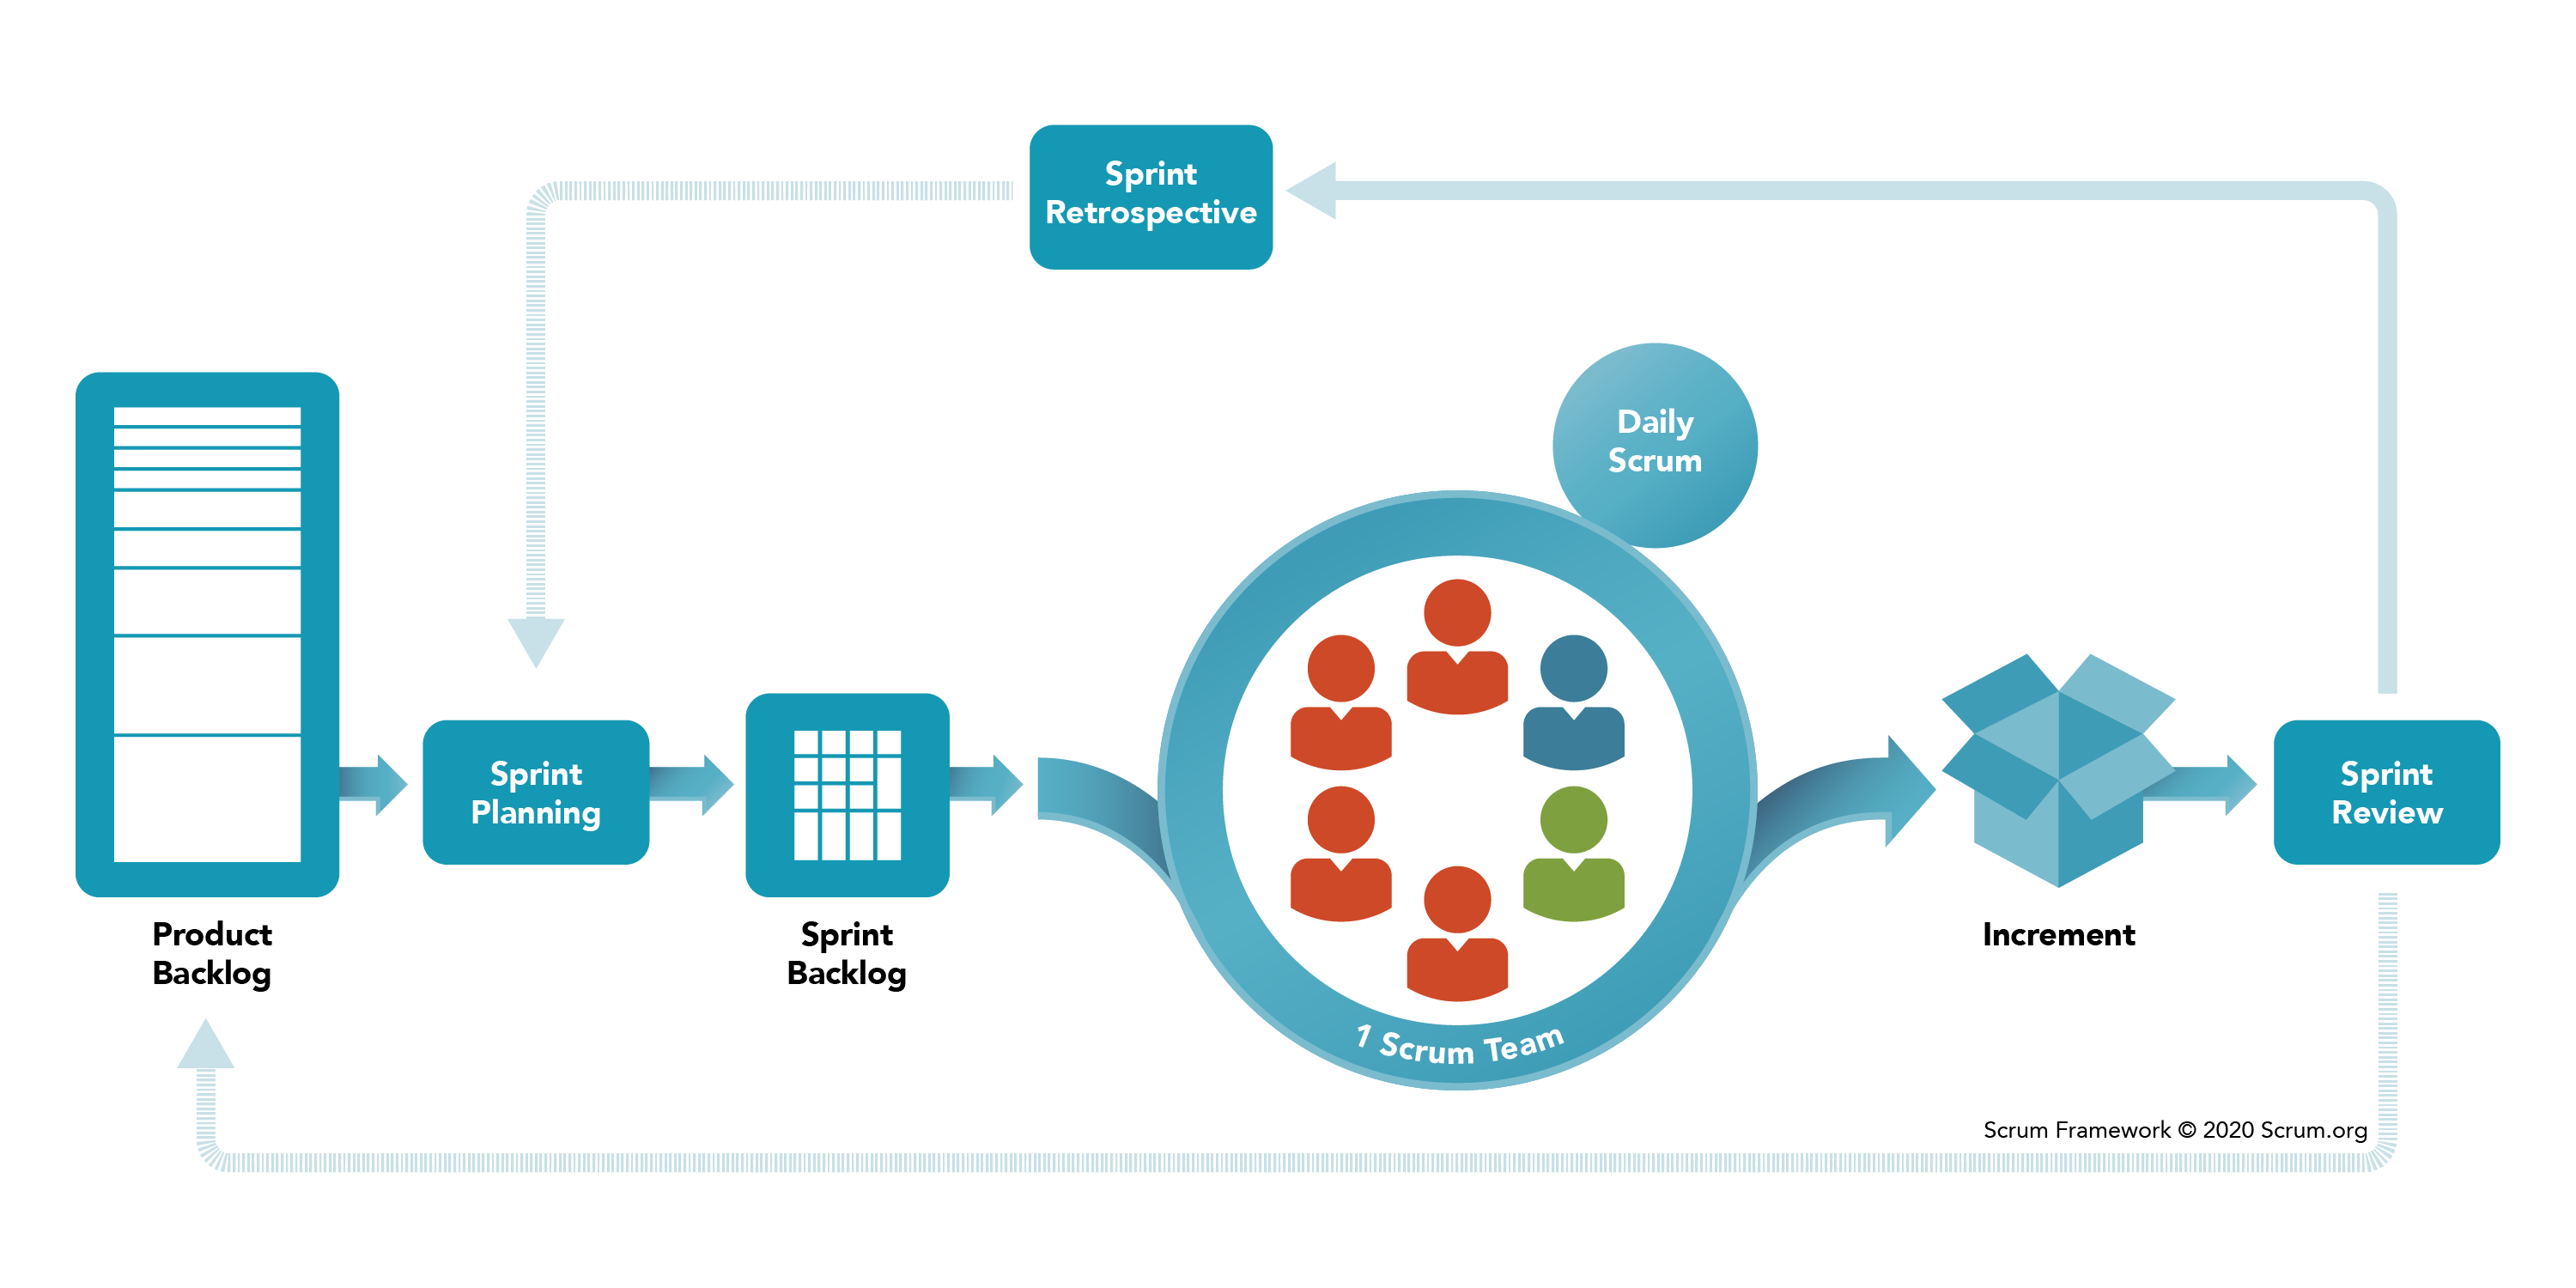
\includegraphics[width=1\textwidth]{scrum}
					\caption{SCRUM Framework}
					\label{fig:scrum}
				\end{figure}
			
				Nel mondo \emph{Agile} sono nati diversi metodi e processi con approcci differenti alla filosofia precedentemente descritta, uno dei quali è \textbf{SCRUM Framework}, il più diffuso ed utilizzato nel mondo dello sviluppo software.
				
				Il termine \textbf{SCRUM} deriva dal gioco del \emph{Rugby}, più precisamente dal pacchetto di mischia, e viene usato come metafora del team di sviluppo che deve lavorare insieme in modo che tutti gli attori del progetto \emph{spingano} nella stessa direzione, agendo come una unica entità coordinata.
				
				Notiamo come non stiamo definendo un processo, ma bensì un \emph{framework}, e come tale si propone come
				collezione di metodologie che sposano la filosofia \emph{Agile} ma che possono essere implementate al meglio delle proprie possibilità, anche con minimi adattamenti.
				
				\emph{SCRUM} si basa sulla teoria dei controlli empirici di analisi strumentale e funzionale di processo, e si basa su alcuni pilastri derivanti da tale teoria:
				\begin{enumerate}
					\item \textbf{Trasparenza}: gli aspetti rilevanti del processo devono essere visibili ai responsabili. Questa trasparenza richiede che venga utilizzato un \emph{linguaggio comune} condiviso da tutti, ed una definizione di
					\emph{done} (finito) condivisa tra gli addetti ai lavori e chi deve accettarlo;
					\item \textbf{Ispezione}: l'uso di SCRUM prevede l'ispezione frequente degli \emph{artefatti} prodotti ed i progressi realizzati verso gli obiettivi stabiliti, individuando precocemente eventuali deviazioni. La frequenza di tali ispezioni deve essere tale da non rallentare il corso dei lavori, e deve essere effettuato da ispettori qualificati;
					\item \textbf{Adattamento}: se durante l'ispezione si trovano difformità oltre i limiti accettabili, bisogna intervenire sul processo stesso e sul materiale prodotto. L'intervento deve essere portato a termine il più velocemente possibile per evitare ulteriori ripercussioni e ridurre al minimo le perdite. Vengono quindi definite quattro occasioni per ispezione e adattamento:
					\begin{itemize}
						\item Sprint Planning Meeting;
						\item Daily Scrum;
						\item Sprint Review;
						\item Sprint Retrospective.
					\end{itemize}.
				\end{enumerate}
			
				\paragraph{Il Team SCRUM}
				In un processo dove si utilizza \emph{SCRUM}, viene definito il team di sviluppo come \emph{Team SCRUM}, formato da diverse figure:
				\begin{itemize}
					\item \textbf{Product Owner}: rappresenta gli stakeholders (cliente), ed è responsabile del valore business del team. Il PO definisce gli \emph{item} (requisiti di prodotto) in base ai bisogni dei clienti (usando \emph{user stories}), assegnando la loro priorità e li inserisce nel \emph{product backlog};
					\item \textbf{Team di Sviluppo}: l'insieme degli sviluppatori responsabili della consegna del prodotto, con incrementi potenzialmente rilasciabili alla fine di ogni \textbf{Sprint}. Il team è composto da un numero di persone che varia da 3 a 9, con competenze cross-funzionali e che si auto-organizza;
					\item \textbf{Scrum Master}: responsabile della rimozione di ostacoli che potrebbero limitare la capacità produttiva del team e quindi di raggiungere gli obiettivi dello \emph{Sprint}. Sebbene possa sembrare un ruolo manageriale,
					lo Scrum Master è solo il supervisore del processo, detta l'autorità relativa alla applicazione delle norme e presiede le riunioni importanti, e funge da protezione al team di sviluppo che può così concentrarsi sullo sviluppo.
				\end{itemize}
			
				\paragraph{Sprint}
				Nello sviluppo \emph{SCRUM}, l'unità base di tempo è chiamato \emph{Sprint}, generalmente di durata di 1-4 settimane. Ogni Sprint inizia con una \textbf{riunione di pianificazione}, e si conclude con una \textbf{riunione di revisione} del raggiungimento degli obiettivi. Durante lo Sprint non è inoltre permesso cambiare gli obiettivi prefissati all'inizio, che verranno quindi tenute in considerazione nell'iterazione successiva.
				
				Al termine di ogni Sprint, il team consegna una versione potenzialmente completa e funzionale del prodotto, contenente gli sviluppi conclusi nello Sprint stesso e quelli dei precedenti già conclusi.
				Le funzionalità da sviluppare in uno Sprint provengono dal \emph{product backlog}, come compilato e prioritizzato dal \emph{Product Owner}, ed una volta inserite nello \textbf{sprint backlog} non possono essere più aggiunte ne rimosse durante il corso dell'iterazione.
				
				\paragraph{Eventi}
				In SCRUM gli eventi vengono sfruttati per \textbf{creare una routine} e ridurre al minimo riunioni al di fuori di quelle definite dal framework stesso, tali eventi sono inoltre inclusi nel timeboxing del processo così da integrarsi al meglio con lo sviluppo stesso senza bloccare il team più del dovuto.
				
					\subparagraph{Sprint Planning}
					All'inizio di ogni Sprint, viene effettuato un meeting volto a pianificare le attività dello stesso e gli obiettivi da conseguire entro la sua conclusione, e coinvolge tutto lo Scrum Team. Al suo interno viene definito lo \emph{sprint backlog} e si ottiene una stima delle tempistiche e risorse necessarie al suo completamento.
					
					\subparagraph{Daily Scrum}
					Ogni giorno durante lo Sprint, viene effettuata una riunione di comunicazione con tutto il team, in cui ogni componente aggiorna gli altri con la sua situazione di sviluppo. Tale meeting viene effettuato nello stesso posto e ora ogni giorno, in un tempo ben definito e ridotto (15 minuti massimo), e viene generalmente effettuato in piedi (da qui il nome \emph{daily standup}).
					
					\subparagraph{Sprint Review}
					Alla fine dello Sprint viene effettuato un meeting volto a ispezionare l'incremento e adattare, se necessario, il \emph{product backlog}. Durante tale riunione il team di sviluppo e gli \emph{stakeholders} collaborano su
					ciò che è stato prodotto durante lo Sprint, viene individuato ciò che è stato "fatto" e non, si discute dei problemi incontrati durante lo sviluppo e il \textbf{Product Owner} discute il \emph{product backlog} fornendo una stima dei tempi di sviluppo futuri.
					
					\subparagraph{Sprint Retrospective}
					Questo meeting fornisce al Team Scrum la possibilità di ispezionare se stesso e creare quindi un piano di miglioramento da attuare nelle prossime iterazioni. Durante tale meeting si analizza l'ultimo Sprint riguardo persone, processi e strumenti, così da identificare i punti di miglioramento e cosa invece ha funzionato correttamente. Lo Scrum Master fornisce un ruolo chiave durante la retrospettiva, incoraggiando il team a migliorarsi, e aiutando a trovare i punti di discussione.
							
			\subsection{Un metodo veloce: eXtreme Programming}
			
				\begin{figure}[h]
					\centering
					
\includegraphics[width=0.5\textwidth]{xp_plan}
					\caption{Iterazione in XP}
					\label{fig:xp_plan}
				\end{figure}
			
				Il metodo di sviluppo denominato \textbf{eXtreme Programming} (abbreviato \textbf{XP}), enfatizza la scrittura di codice di qualità e la rapidità di risposta ai cambiamenti dei requisiti. Rispetto a \emph{SCRUM Framework}, XP si basa su elementi chiave totalmente differenti tra cui il \emph{Pair Programming}, lo \emph{Unit Testing} e il \emph{Refactoring}, oltre che la necessità di scrivere solo codice strettamente necessario nel modo più semplice possibile.
				
				\paragraph{Le 12 Regole di XP}
				\begin{enumerate}
					\item \textbf{Feedback}
						\begin{enumerate}
							\item \emph{Pair Programming}: due programmatori lavorano assieme sulla stessa macchina, uno di essi è il \emph{driver} che scrive il codice e l'altro è il \emph{navigator} che ragiona sull'approccio;
							\item \emph{Planning Game}: una riunione di pianificazione che avviene una volta per iterazione;
							\item \emph{Test Driven Development}: i test automatici (unit e acceptance) vengono scritti \emph{prima} del codice;
							\item \emph{Whole Team}: il cliente non è colui che finanzia, ma colui che utilizza il sistema, motivo per cui deve essere sempre presente e disponibile per verifiche;
						\end{enumerate}
					\item \textbf{Continuous Process}
						\begin{enumerate}
							\item \emph{Continuous Integration}: integrare continuamente i cambiamenti nel codice eviterà problemi più avanti nel progetto;
							\item \emph{Refactoring}: riscrivere il codice senza cambiarne le funzionalità, rendendolo più semplice e generico;
							\item \emph{Small Releases}: il software viene rilasciato frequentemente con incrementi ridotti ma che portano valore concreto;
						\end{enumerate}
					\item \textbf{Shared Comprehension}:
						\begin{enumerate}
							\item \emph{Coding Standards}: utilizzare uno standard di scrittura preciso e condiviso, da rispettare lungo tutto il corso del progetto;
							\item \emph{Collective Code Ownership}: ognuno è responsabile di tutto il codice, quindi chiunque contribuisce alla sua stesura;
							\item \emph{Simple Design}: seguire un approccio \emph{"simple is better"} durante la progettazione;
							\item \emph{System Metaphor}: descrivere formalmente il sistema mediante metafore, rendendolo più semplice da comprendere in poche parole;
						\end{enumerate}
					\item \textbf{Programmers Wellbeing}:
						\begin{enumerate}
							\item \emph{Sustainable Pace}: gli sviluppatori non dovrebbero lavorare oltre un numero di ore stabilite settimanalmente (generalmente 40).
						\end{enumerate}
				\end{enumerate}
			
			Una delle differenze sostanziali con altri metodi \emph{Agile}, è il focus sul \textbf{metodo di sviluppo} piuttosto che sul processo in se. Extreme Programming si prefigge quindi di ottimizzare al meglio lo sviluppo del software mediante tecniche e metodiche applicabili dagli sviluppatori stessi, senza necessità di utilizzo di figure esterne o di guide, e propone diversi concetti che sono stati ripresi in buona parte dalle metodologie \emph{DevOps} che andremo a descrivere.
	
		\section{Metodologie di Sviluppo \emph{Agile}: DevOps}
		
			In un mondo dove lo sviluppo \emph{Agile} prende sempre più piede, si è reso necessario trovare un qualcosa che potesse migliorare notevolmente i processi già in atto, attuando delle modifiche sostanziali al come i team di sviluppo lavorano tra di loro e a quale livello di integrazione.
			
			In particolare ciò di cui ci si è accorti nel tempo è il livello di isolamento che ogni team attua al proprio lavoro, in particolare tra i team di Development e Operations, consci però che un software è fatto di entrambe le parti che non possono prescindere dall'altra.
		
			\subsection{Un po' di storia}
				
				Se qualcuno chiedesse da dove ebbe \textbf{origine} il termine \textbf{DevOps}, la risposta sarebbe \emph{Patrick Debois}. Quando fu un IT Consultant in Belgio, nel 2007, Debois lavorò ad un progetto per il governo belga riguardo una migrazione di un data center dove fu in carico del testing dei sistemi. Durante questo periodo si rese conto come stesse spendendo molto tempo tra il mondo dello sviluppo (Development) e delle Operations.
				
				Nel 2008, durante una conferenza riguardo l'\emph{Agile}, \emph{Andrew Shafer} fece una sessione riguardo l'\emph{Agile Infrastructure} dove solo \emph{Patrick Debois} ne prese parte. Nel corso dell'anno crearono un gruppo dove poter discutere di come risolvere questo distaccamento tra il mondo Development e Operations, cosa che si evolse nell'Ottobre 2009 quando crearono un evento per avvicinare sviluppatori e system administrators che chiamarono \textbf{DevOpsDays}, unendo così le parole Development e Operations per la prima volta.
				
				Da allora il termine \textbf{DevOps} continuò ad essere usato su Twitter, fino ad arrivare alla accezione odierna.
			
			\subsection{Un metodo ed un'etica}
			
				Applicare un metodo e delle pratiche \emph{DevOps} non vuol dire solamente utilizzare determinati tool o effettuare certe azioni, ma il concetto si estende a ciò che può essere definito \textbf{una etica da applicare} a livello aziendale o progettuale a cui tutti gli attori coinvolti devono aderire per trarne il massimo beneficio.
				
				\begin{figure}[h]
					\centering
					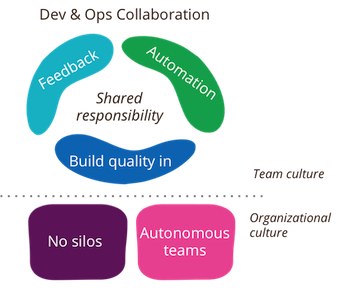
\includegraphics[width=0.5\textwidth]{devops_culture}
					\caption{La cultura DevOps}
					\label{fig:devops_culture}
				\end{figure}
				
				I principi guida dell'etica \emph{DevOps} includono un cambiamento culturale pervasivo, un metodo per misurare le prestazioni, automazione estesa e condivisione, si potrebbe anche definire il \emph{DevOps} come l'approccio più moderno al classico \textbf{Application Lifecycle Management} (ALM). Questi principi possono essere riassunti in un framework chiamato \textbf{CALMS}, dall'acronimo \emph{Culture - Automation - Lean Flow - Measurement - Sharing}, termine coniato da \emph{Jez Humble}, co-autore del libro \emph{The DevOps Handbook}.\\*
				
				I team di sviluppo e di operations si uniscono e diventano \textbf{responsabili dell'intero processo produttivo}, dallo sviluppo delle feature alla messa in produzione del software fino alla manutenzione e al monitoring dello stesso. L'approccio all'intero ciclo di vita del software da parte di entrambi i team permette di avvicinare gli sviluppatori a ciò che realmente vuole l'utente, acquisendo anche feedback dalle fasi finali e aumentando la trasparenza attraverso tutti gli attori coinvolti.
			
			\subsection{Obiettivi delle pratiche DevOps}
			
				La principale caratteristica delle pratiche \emph{DevOps} è la \textbf{collaborazione} tra i ruoli di Development e Operations.
				Per supportare tale collaborazione si necessita una attitudine di \emph{shared responsibility}, è facile infatti perdere interesse per una materia o l'altra se ci sono team separati a gestirle senza comunicazione ne necessità di interazione tra loro, faccenda diversa quando invece il team di sviluppo controlla tutto il processo dall'inizio alla fine comprendendo processi di operations come \textbf{deployment} e \textbf{monitoring} in produzione.\\*
				
				Per applicare tali pratiche è inoltre indispensabile un cambiamento organizzativo all'interno dei team, \textbf{non devono esserci separazioni tra Development e Operations} sia di locazione sia di argomenti trattati, ognuno deve essere responsabile dei successi e fallimenti di un sistema puntando sempre più ad eliminare le divergenze tra i due team citati, arrivando ad un tutt'uno.\\*
				
				Un altro cambiamento sostanziale, derivante dalla filosofia \emph{Agile}, è la necessità di \textbf{team autonomi}, ovvero che non necessitano la presenza costante di figure manageriali ne di processi complessi grazie al quale si possano fare determinate decisioni. Ciò si traduce in una crescente \textbf{fiducia} nelle decisioni prese dal team, ed una gestione dei processi più snello che permetta di non rallentare i lavori per colpa dell'introduzione di azioni solo managing-oriented.\\*
			
				Questi cambiamenti a livello culturale, pratico e metodologico si traducono in risultati tangibili a livello di business, e non solo tecnico:
				\begin{itemize}
					\item Adozione di processi \emph{Agile} facilitata;
					\item Velocità di rilascio notevolmente aumentata (deliverables);
					\item Velocità di risposta ai cambiamenti aumentata e facilitata, aumento del livello di feedback;
					\item Team \emph{cross-skilled} e \emph{self-improved} per costi ridotti e performance migliorate;
					\item Qualità del prodotto notevolmente aumentata, grazie al testing estensivo.
				\end{itemize}
			
				Nel \textbf{"Atlassian Survey on DevOps Trends"} del 2020, il \textbf{99\%} degli intervistati ha espresso che l'utilizzo di pratiche DevOps ha portato un \textbf{impatto positivo} nella loro realtà, tra cui il 78\% ha dovuto imparare nuove skill per utilizzare tali pratiche ma al contempo al 48\% ha contribuito anche ad un aumento di salario grazie al self-improvement.
			
				\begin{figure}[H]
					\centering
					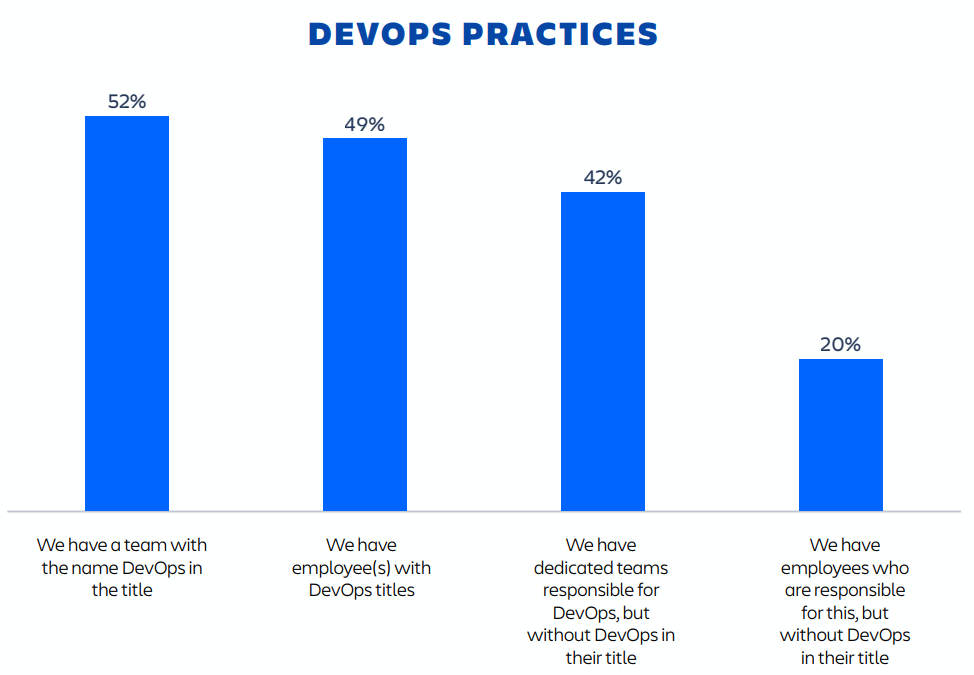
\includegraphics[width=0.65\textwidth]{atlassian_devops_practices}
					\caption{Atlassian Survey - Adozione DevOps}
					\label{fig:atlassian_devops_practices}
				\end{figure}

				I vantaggi del \emph{DevOps} sono inoltre chiari da questo survey, dove il 61\% degli intervistati ha affermato che applicare tali pratiche ha migliorato la qualità dei prodotti finali, e per il 49\% ha velocizzato il \emph{time-to-market} e la consegna di \emph{deliverables} anche parziali in meno iterazioni. Nei fattori di successo nell'implementazione di pratiche \emph{DevOps} si trovano i \textbf{tool corretti} e le \textbf{persone giuste}, che possano collaborare e performare ottimamente con una ottima abilità di problem-solving.
				
				\begin{figure}[H]
					\centering
					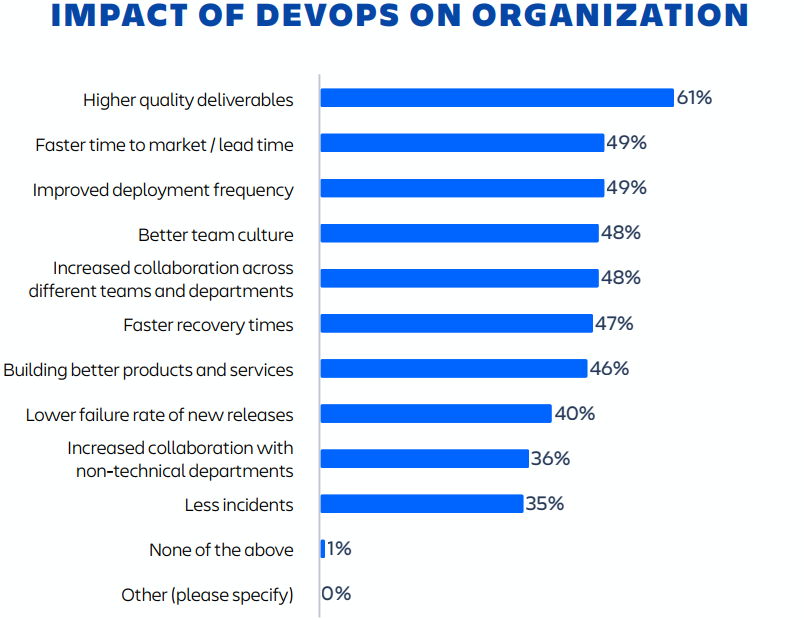
\includegraphics[width=0.7\textwidth]{atlassian_devops_impact}
					\caption{Atlassian Survey - Impatto sul Business}
					\label{fig:atlassian_devops_impact}
				\end{figure}
				
				Il rovescio della medaglia risiede nella difficoltà di implementazione dei metodi \emph{DevOps}, dove ben l'85\% ritiene di aver trovato problemi o difficoltà, e vede come principali fattori problematici la mancanza di \emph{skills} dei propri dipendenti, la presenza di infrastrutture \emph{legacy} e difficilmente mantenibili ed estensibili, e una difficoltà nell'aggiustare la \emph{cultura} aziendale radicata nel tempo.\\*
				
				Infine, riprendendo i pilastri del \emph{DevOps}, ritroviamo ciò che viene definito un "metodo" per misurare le performance e i risultati di tali pratiche, sia tecniche che business. Nel survey il 74\% ritiene di avere un metodo efficace per misurare l'impatto di ciò che viene implementato (generalmente basato sulla velocità di deployment o delivery), e ben il 97\% si definisce soddisfatto del modo in cui stanno misurando gli effetti delle pratiche.
			
			\subsection{Processo di Riferimento}
				
				\begin{figure}[H]
					\centering
					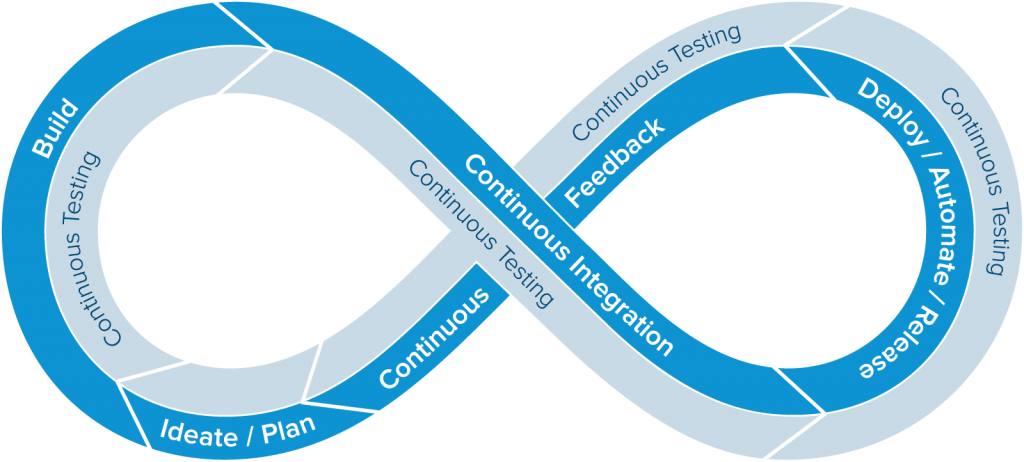
\includegraphics[width=0.8\textwidth]{devops_cycle}
					\caption{Processo DevOps-based}
					\label{fig:devops_cycle}
				\end{figure}
	
				Una tipica modellizzazione del processo \textbf{DevOps-oriented} è definita da un simbolo dell'infinito, che riflette ciò che abbiamo introdotto con le metodologie \emph{Agile} e lo sviluppo ad iterazioni incrementali. Il processo finale ha come scopo la massima agilità ed automazione durante tutte le fasi di sviluppo e deployment, permettendo un continuo avvicinamento tra i ruoli di development e operations in ogni fase dello stesso.
				
				Il processo \emph{DevOps} deve essere implementato unendo cultura, metodiche e strumenti in un ambiente coeso, basandosi sempre su processi di tipo \emph{Agile} o sfruttando framework che permettano di implementarlo in modo efficace.\\*
				
				Le sue fasi sono così definite:
				\begin{itemize}
					\item \textbf{Ideate/Plan}: i tasks vengono organizzati, pianificati nell'iterazione (Sprint), e vengono inizializzati i tools di gestione del processo (Boards, Documentazione, SCM, e molti altri). L'idea di base è poter sfruttare il concetto di \textbf{user story} introdotto nelle metodologie \emph{Agile}, così da permettere sia a "dev" che "ops" di comprendere la feature in modo semplice;
					\item \textbf{Code/Build}: il codice viene scritto e controllato mediante utilizzo di \textbf{Code Reviews}, che una volta approvata viene unita alla branch principale del VCS scelto. Il codice deve poi essere compilato (buildato) per controllare la sua correttezza e produrre i primi artefatti di debug;
					\item \textbf{Continuous Integration}: una fase cruciale che si mixa con quella di build, il codice viene testato ed integrato con l'attuale codebase prima del merge sulla branch principale, evidenziando eventuali errori nei test automatici o nelle dipendenze dei sistemi. Questo processo è continuo e automatico per ogni commit o Code Review creati, e vengono sfruttati tool dedicati a velocizzarlo e implementarlo con successo;
					\item \textbf{Deploy/Release}: una volta passata la fase di \emph{CI}, il codice è pronto per il rilascio. Questa fase viene automatizzata mediante processi di \textbf{Continuous Delivery} e \textbf{Continuous Deployment} (uno conseguente all'altro), ovvero la build degli artefatti finiti e pronti al rilascio viene "inviata" ad un sistema centralizzato di storage, per poi essere deployato automaticamente sulla infrastruttura ospitante.
					\item \textbf{Continuous Feedback}: la fase più operations-oriented del processo, il codice deployato deve essere controllato mediante sistemi di \textbf{Monitoring}, creando così delle metriche di performance ed implementando un flusso di \textbf{Observability}.
				\end{itemize}
				
				Nella nostra analisi ci concentreremo sul descrivere le fasi centrali del processo di \emph{DevOps}, ovvero quelle che coinvolgono attivamente sempre tutto il team e che vengono effettuate più spesso durante le iterazioni del processo, ovvero \textbf{Continuous Integration}, \textbf{Continuous Delivery} e \textbf{Continuous Deployment}.
				
				\subsubsection{Continuous Integration}
				
					La \emph{Continuous Integration (CI)} è la pratica di automatizzare ed integrare i cambiamenti del codice da parte di molte fonti (sviluppatori) in una singola codebase. Viene definita come una delle pratiche fondamentali del processo \emph{DevOps} e permette agli sviluppatori di scrivere, integrare e testare velocemente le feature utilizzando dei sistemi di automazione che controllano la correttezza del software on-demand.
					
					\begin{figure}[h]
						\centering
						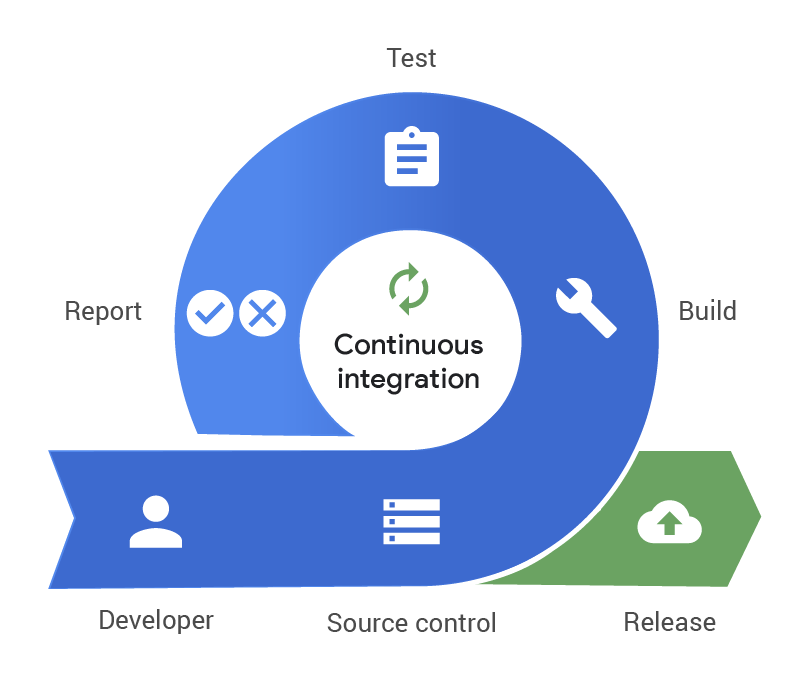
\includegraphics[width=0.5\textwidth]{devops_ci}
						\caption{DevOps - Continuous Integration}
						\label{fig:devops_ci}
					\end{figure}
					
					Per implementare un sistema di \emph{CI}, sono necessari:
					\begin{enumerate}
						\item Un sistema di repository versioning (generalmente Git);
						\item Un codice auto-testante, ovvero che contiene test automatici (Unit, Integration, E2E);
						\item Un ambiente di test unificato e indipendente dalle macchine degli sviluppatori;
						\item Un tool che gestisca il processo (Jenkins, Gitlab CI, e molti altri);
						\item Massima visibilità dei risultati prodotti dal processo (test, errori, dipendenze);
					\end{enumerate}
					
					Il processo prevede diverse fasi che includono la cooperazione tra sviluppatori e un tool che gestisca il processo stesso, implementando le sue fasi automatiche:
					\begin{enumerate}
					    \item \textbf{Developer}: lo sviluppatore scrive il codice della feature necessaria, assieme al codice è necessario scrivere \textbf{test automatici} sia di tipo \emph{unit} che \emph{integration}. La presenza di questi test valuterà la qualità finale del processo di integrazione;
					    \item \textbf{Source Control}: le modifiche alla code base vengono inserire in un sistema di version control (es. Git), generalmente usando \emph{branch} separate dalla \emph{master};
					    \item \textbf{Build}: il tool di CI avvia una build automatica comprendente le modifiche aggiunte dallo sviluppatore al codice principale. L'ambiente di build è controllato ed unificato, così da ridurre al minimo la variabilità;
					    \item \textbf{Test}: il tool di CI avvia il \emph{testing automatico} sulla codebase, che comprende sia \emph{unit tests} che \emph{integration tests};
					    \item \textbf{Report}: il risultato dei test avviati viene visualizzato ed analizzato all'interno del tool di CI, le parti coinvolte vengono informate dello status dell'integrazione e di eventuali fallimenti.
					\end{enumerate}
					
					Questo processo viene iterato fino alla fine dello sviluppo della feature, ogni singola modifica sarà quindi controllata dal sistema e solo se tutto passerà i test automatici allora si potrà integrare con successo il codice nuovo nella codebase principale (generalmente la \emph{master} branch). Una delle pratiche comuni durante l'utilizzo di una pipeline di CI, è l'introduzione del \textbf{TDD} come visto nei principi di \emph{XP}, ottenendo così una copertura completa delle righe di codice rispetto ai test scritti.\\*
					
					Una estensione naturale del processo di \emph{CI} si presenta con l'introduzione dell'\textbf{analisi statica e dinamica} del codice mediante lo stesso tool o altri tools dedicati. Questa analisi permette di ridurre l'impatto del \emph{technical debt} in fasi precoci dello sviluppo, fornendo allo sviluppatore uno sguardo veloce in cosa potrebbe potenzialmente causare bug o problemi di mantenibilità nel lungo termine e risolverli in fasi precoci dello sviluppo.
				
				\subsubsection{Continuous Delivery}
					
					Se con la \emph{Continuous Integration} abbiamo descritto un processo in continuo utilizzo attivo da parte di tutti gli sviluppatori, il processo di \emph{Continuous Delivery} può essere approcciato con diverse metodologie e tempistiche in base al proprio ciclo di rilascio del software.\\*
					
					Nella fase finale dello schema di CI, troviamo la fase di \textbf{Release}, generalmente preceduta da ciò che viene definita la \textbf{delivery degli artefatti software}, ovvero la build automatica e l'invio con storage dei prodotti finali pronti all'uso e alla release in una fase successiva. Un tipico artefatto in output di un sistema di CD è un \emph{container}, unità che permette poi di semplificare anche il deployment successivo in ambienti diversi.\\*
					
					\begin{figure}[ht]
						\centering
						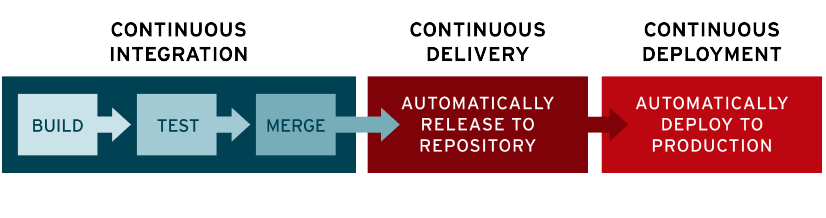
\includegraphics[width=0.8\textwidth]{ci_cd_flow}
						\caption{DevOps - Processo Completo}
						\label{fig:ci_cd_flow}
					\end{figure}
					
					L'obiettivo di questa processo è di avere una collezione di artefatti software \textbf{pronti alla release} in qualsiasi momento, così da velocizzare il processo di deployment successivo. L'evento che può triggerare una build automatica potrebbe essere un \emph{tag} sul \emph{repository}, oppure un trigger manuale attraverso un tool dedicato, oppure la semplice fine di una iterazione di sviluppo (Sprint) dopo la quale si necessita di inviare il software prodotto al cliente o di "congelare" la codebase attuale.
				
				\subsubsection{Continuous Deployment}
				
					Un flusso di CI/CD maturo sfocia in quello che viene definito \emph{Continuous Deployment}, ovvero l'automazione dell'ultimo tratto che porta alla fruizione automatica delle nuove feature sviluppate, direttamente in un ambiente di produzione finale.\\*
					
					Questo processo fa forte affidamento nella solidità e precisione dei precedenti flussi, dove il testing deve necessariamente essere estensivo al punto di garantire un rilascio in produzione senza problemi, che possa così essere automatizzato senza preoccupazioni. Generalmente l'uso del deployment automatico porta al \emph{time-to-market} più veloce possibile, e una feature potrebbe in pochi minuti essere operativa dopo l'esser stata sviluppata e testata.\\*
					
					Una feature indispensabile a supporto del \emph{Continuous Deployment} è la possibilità di effettuare dei \textbf{rollback} senza impattare il resto del sistema ed in modo automatico in caso di fallimenti non previsti. Questi avvisi di "non funzionamento" devono necessariamente provenire da un sistema di \emph{monitoring} che permetta di valutare errori e prestazioni del software in una fase post-release.
					
	    \section{\emph{DevOps}: l'impatto sul business}
	        
	        I dati pubblicati dal \emph{State of DevOps Report} redatto da \textbf{Puppet} e \textbf{CircleCI}, due dei più grandi strumenti utilizzati in ambito DevOps, rivelano gli impatti significativi che tali pratiche hanno portato in ambienti business ed IT-oriented.
	        
	        Dopo aver intervistato oltre 2500 partecipanti, nonostante le condizioni lavorative dell'anno 2020 dovute alla pandemia globale di COVID-19, sono emersi alcuni punti chiave nel mondo DevOps:
	        
	        \paragraph{DevOps come Piattaforma}
	        Con la crescente necessità di unificare i team, si sono creati dei team "di prodotto" che si occupano di tutto il ciclo di vita di un software. La nascita di molti team separati rischia di creare diversità e problematiche per l'uso di tools, pratiche e processi diversi.\\*
	        
	        Molte realtà si sono quindi adattate nel creare un \textbf{team di platform} che possa gestire tutti questi aspetti per tutti i team in modo univoco, unificando i processi e strumenti, e snellendo il peso dell'uso degli stessi da parte di ogni sviluppatore, che prende parte attivamente al processo ma non si trova in mezzo a decisioni burocratiche che potrebbero rallentare il lavoro.
	        
	        Oltre il 63\% delle aziende ha una piattaforma interna comune, e il 77\% ha 3 o più servizi all'interno della stessa. Da denotare inoltre il grado di utilizzo di tale piattaforma, tendente sempre più verso il massimo, ma ancora più del 50\% non la sfrutta a dovere (< 50\% degli sviluppatori in azienda).\\*
	        
	        Trattare la piattaforma DevOps come un \textbf{prodotto} è una delle core features di una azienda di successo, quindi mantenere dei requisiti per gli stakeholders con una roadmap, gestire l'onboarding nella stessa in modo efficace ed avere una figura di riferimento come un Product Manager che possa analizzare i requisiti e il "mercato".
	        
	        \begin{figure}[h]
				\centering
				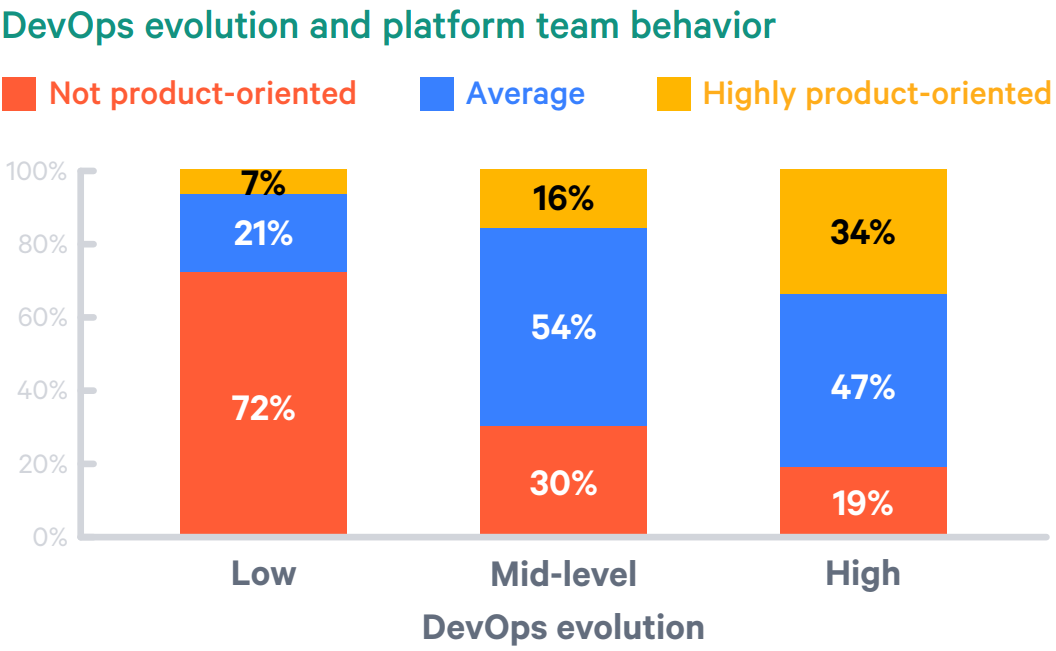
\includegraphics[width=0.6\textwidth]{devops_product_evolution}
				\caption{State of DevOps 2020 - Platform Behaviour}
				\label{fig:devops_product_evolution}
			\end{figure}
	        
	        \paragraph{Cambiamenti nel Management}
	        Se una azienda non è in grado ancora di trattare il DevOps come una piattaforma unica, il metodo più efficace per velocizzare la delivery del software è un cambiamento di \textbf{cultura ed etica} a livello di management.
	        
	        \begin{figure}[h]
				\centering
				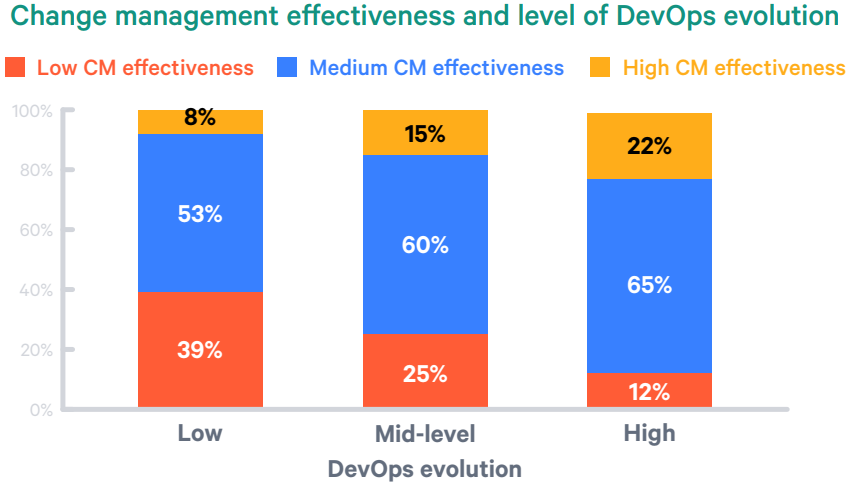
\includegraphics[width=0.7\textwidth]{devops_change_mgmt}
				\caption{State of DevOps 2020 - Change Management}
				\label{fig:devops_change_mgmt}
			\end{figure}
	        
	        Si sono visti 4 approcci principali al cambiamento interno:
	        \begin{itemize}
	            \item \emph{Ad-Hoc}: automazione ridotta, risk-mitigation ridotta, improntata allo small/mid market e adattabilità ridotta nel tempo;
	            \item \emph{Governance Focused}: automazione ridotta, risk-mitigation ridotta, improntata al mid/large market e dipendente da politiche aziendali interne;
	            \item \emph{Engineering Driven}: alto livello di automazione, risk-mitigation estesa, improntata allo small/mid market con alta adattabilità nel tempo;
	            \item \emph{Operationally Mature}: alto livello di automazione, risk-mitigation estesa, improntata al mid market specificatamente e dipendente dalle politiche aziendali interne.
	        \end{itemize}
	
	        Si è anche notato come l'approccio più governance-oriented e quindi più rispondente alle politiche aziendali preesistenti, rallenti notevolmente i processi e renda inefficiente il lavoro allontanandosi così dal concetto di \emph{Agile Development}. Un alto livello di automazione al contrario, rende gli addetti ai lavori molto confidenti nel cambiamento in atto, riduce i rischi dovuti a problematiche di ogni natura e assicura un \emph{time-to-market} nettamente migliore.\\*
	
	        Ogni approccio presenta comunque un lato negativo, ad esempio le aziende \emph{Operationally Mature} presentano una tolleranza al rischio molto bassa, mentre le \emph{Engineering Driven} si sentono limitate dalla loro architettura applicativa. Non esiste l'approccio perfetto in nessuna delle 4 casistiche, ma i driver di successo sono sicuramente un processo più snello, meno governance e un livello di automazione tale per cui la confidenza possa rimanere alta sia nello sviluppo che nel management.
	
	        \begin{fquote}[Kent Beck - Extreme Programming Explained: Embrace Change]
    		 	The problem isn't change, per se, because change is going to happen; the problem, rather, is the inability to cope with change when it comes.
    	 	\end{fquote}
	
		    \subsection{Il \emph{ROI} del DevOps}
		
		        Una tipica domanda che qualsiasi leader aziendale si pone quando si approccia alle metodologie \emph{DevOps} è: quanto ritorno positivo (economico e tecnico) mi comporta, ed in quanto tempo?
		        Risulta chiaro dalla teoria come l'uso di queste pratiche comporti uno sviluppo più \emph{Agile}, rischi ridotti nel medio-lungo termine e \emph{time-to-market} più veloce, ciò che manca è una metrica per valutare quantitativamente l'impatto sull'azienda e sui prodotti offerti dalla stessa.\\*
		        
		        Il calcolo del ROI si basa principalmente sui guadagni attesi rispetto alle spese, solitamente espressi in guadagni economici ma spesso scartando il guadagno in fattore \emph{tempo}, uno dei punti di forza di queste pratiche. L'analista \textbf{Michael Cote} ha affermato come definire quantitativamente il ROI del \emph{DevOps} sia contemporaneamente "assurdo e fondamentale" per la sua complessità in fatto di variabili in gioco, che renderebbe la stima estremamente imprecisa e mai veritiera, quindi difficilmente stimabile.\\*
		        
			    Esiste però un indicatore numerico che può riflettere il principale vantaggio del \emph{DevOps}, ovvero il cosiddetto \textbf{MTTR} - \emph{mean time to repair} - il tempo impiegato a rilevare e risolvere gli errori del software o del progetto in se, proporzionale al tempo di inattività o stallo del ciclo di sviluppo, valore che diminuisce con meno \emph{deployments} effettuati.
			    
			    \begin{figure}[ht]
    				\centering
    				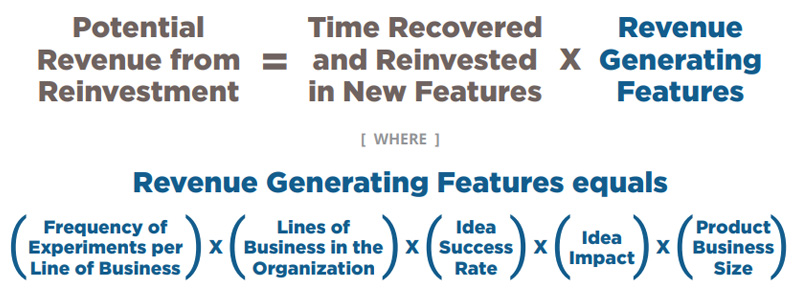
\includegraphics[width=0.7\textwidth]{devops_roi}
    				\caption{DevOps - Impatto sul ROI}
    				\label{fig:devops_roi}
			    \end{figure}
			    
			    Cosa si può dire riguardo l'impatto nel lungo e medio termine? CloudMunch, per esempio, misura annualmente valori come il tempo di deployment, il livello di automazione di task ripetitivi e del supporto, e moltiplicandoli per il costo medio di uno sviluppatore all'ora ricava una misura potenziale del ROI del \emph{DevOps} nel corso di un anno solare. Esistono diversi esempi di metodologie diverse, tutte però adattate alla propria realtà e mai un indicatore preciso ed univoco del vero ROI.\\*
			    
			    Non vi è ombra di dubbio sulla difficoltà di calcolo del ROI, specialmente per un processo che tutt'ora è in fase di adozione e non è improntato tanto sull'aumento del guadagno economico ma più sul velocizzare quello previsto dal progetto. Secondo \emph{Patrick Debois}, uno dei padri fondatori del movimento \emph{DevOps}, dovremmo pensare il ROI come una "realizzazione più veloce dei benefici" già previsti dal progetto in se, accorciando così i cicli di sviluppo che possono essere ridotti e raggiungere gli obiettivi prima.
	
	\chapter{Sviluppo ed Automazione su Cloud}
	
	\section{Perchè il Cloud?}
	
	\section{\emph{Infrastructure-as-a-Code}}
	
	\section{\emph{Configuration-as-a-Code}}
	
	\section{Containers ed ambienti controllati}
	
	\chapter{Analisi del Processo di Sviluppo}
	
	\section{Struttura del Progetto}
	
	\section{Il processo di sviluppo}
	
	\section{Requisiti e KPI}
	
	\section{Il processo DevOps}
	
	\subsection{Architettura High-Level e Fasi}
	
	\subsection{Gestione del Codice}
	
	\subsection{Pull Requests e Code Review}
	
	\subsection{Continuous Integration}
	
	\subsubsection{Test Automation}
	
	\subsubsection{Code Analysis}
	
	\subsection{Continuous Delivery}
	
	\subsubsection{Build Automation}
	
	\subsubsection{Artifacts Delivery}
	
	\subsection{Deployment}
	
	\section{Tecnologie e Strumenti}
	
	\subsection{SCM: Git}
	
	\subsection{Build System: Bazel}
	
	\subsection{Cloud Provider: AWS}
	
	\subsection{PR Management: Phabricator ed Arcanist}
	
	\subsection{CI/CD: Jenkins}
	
	\subsection{Code Analysis: SonarQube}
	
	\chapter{Tecnologie di Background}
	
	\section{Cloud Provider: \emph{AWS}}
	
	\section{Infrastructure-as-a-Code: \emph{Terraform}}
	
	\section{Configuration-as-a-Code: \emph{Ansible}}
	
	\section{Container Engine: \emph{Docker}}
	
	\chapter{Architettura Cloud}
	
	\section{Diagramma Architetturale}
	
	\section{Configurazione di Phabricator}
	
	\section{Configurazione di Jenkins}
	
	\subsection{Agent su AWS EC2}
	
	\subsection{Agent macOS On-Premise}
	
	\section{Configurazione di SonarQube}
	
	\section{Creazione ambiente di build con Docker}
	
	\chapter{La Pipeline di CI}
	
	\section{Tecnologie e Strumenti}
	
	\subsection{Phabricator ed Arcanist: un flusso controllato}
	
	\subsection{Jenkins: il motore del processo}
	
	\subsection{Docker: ambiente di testing unificato}
	
	\subsection{SonarQube: controllo qualità}
	
	\section{Le fasi della Pipeline}
	
	\section{Analisi del Codice}
	
	\subsection{Quality Gates}
	
	\subsection{Code Coverage}
	
	\subsection{Risposta a cambiamenti nella qualità}
	
	\section{Risultati di Testing e QA}
	
	\chapter{La Pipeline di CD}
	
	\section{Tecnologie e Strumenti}
	
	\subsection{Jenkins: il motore del processo}
	
	\subsection{Docker: ambiente di build unificato}
	
	\section{Le fasi della Pipeline}
	
	\section{Analisi delle Vulnerabilità}
	
	\section{Risultati}
	
	\chapter{Conclusioni}
	
	\section{Obiettivi Raggiunti}
	
	\section{Risultati su Requisiti e KPI}
	
	\section{Evoluzioni Future}
	
	\section{Considerazioni Personali}
	
\end{document}